 \section{Results}\label{sec:results}
\begin{figure}[!htb]
\centering
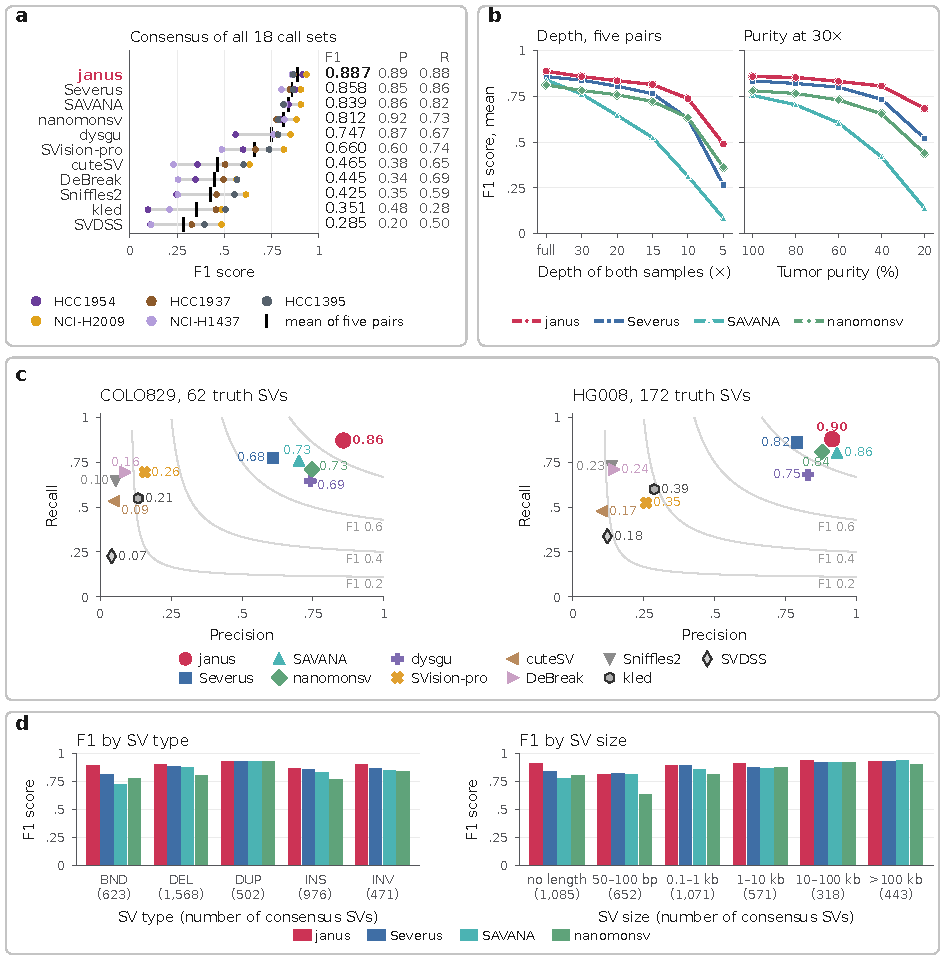
\includegraphics[width=157mm]{figures/fig_accuracy.pdf}
\caption{Accuracy of \tool and the other callers. (a) F1 score of the 11 PacBio HiFi call sets per CASTLE pair (dots) and the mean over pairs (bar), against the consensus of all 18 call sets (P, precision; R, recall). (b) Mean F1 score at reduced depth (left) and purity (right). (c) Precision and recall on COLO829 (left) and HG008 (right), with curves of equal F1 score. (d) F1 score by SV type (left) and size (right), five pairs pooled; inversions include inverted junctions; first size class: SVs without length; consensus SVs in parentheses.}
\label{fig:castle}
\end{figure}

We evaluated \tool using both real and simulated sequencing datasets (Section~\ref{supsec:datasets}).
For comparison, we ran competing PacBio HiFi-based callers using minimap2~\cite{Li_2018} and SAMtools~\cite{samtools} alignments generated from identical read sets (Section~\ref{supsec:tools}) and constructed consensus truth sets using Minda~\cite{minda} (Section~\ref{supsec:consensus}).
Sections~\ref{supsec:simgen} and~\ref{supsec:simeval} detail the simulated dataset generation and truth-set construction.
To assess significance, we computed 95\% bootstrap confidence intervals~\cite{efron} for the F1 score differences between \tool and the best other caller across 2,000 resamples (sampling consensus SVs with replacement for recall and candidate calls for precision).



\subsection{Accuracy analysis on real tumor--normal pairs}\label{sec:accuracy}

We first evaluated \tool on five PacBio HiFi tumor--normal cell line pairs from the CASTLE panel~\cite{severus,deepsomatic} (Table~\ref{suptab:castle}). Lacking a curated ground truth, the panel provides an 11-call-set Minda~\cite{minda} consensus requiring support from at least two technologies and four callers across PacBio HiFi, ONT, and Illumina~\cite{severus,nanomonsv,manta,svaba,gripss,sniffles2,savana}. Because that consensus includes only four of the ten HiFi callers evaluated here, we expanded the truth set to 18 call sets by incorporating \tool, our runs of all ten HiFi callers (Severus, SAVANA, nanomonsv, Sniffles2, dysgu~\cite{dysgu}, SVision-pro~\cite{svisionpro}, cuteSV~\cite{cutesv}, DeBreak~\cite{debreak}, kled~\cite{kled}, and SVDSS~\cite{svdss}; Section~\ref{supsec:tools}), and the panel's seven ONT and Illumina sets. To ensure unbiased benchmarking, we retained the two-technology requirement, raised the caller threshold to six, and applied uniform Minda parameters (500\,bp tolerance, $\ge$50\,bp length; Section~\ref{supsec:consensus}). We trained the classifier on the consensus of the 17 call sets other than \tool, built with the same criteria (Section~\ref{supsec:classifier}).

Using leave-one-out cross-validation over the five CASTLE pairs (Section~\ref{supsec:classifier}), \tool achieved the highest mean F1 score (0.887) against the 18-caller consensus, in which all callers count equally, ranking first in four pairs and trailing only the ONT call set of Severus on HCC1395 (Table~\ref{suptab:castle}, Fig.~\ref{fig:castle}a, Table~\ref{suptab:allwith}, Fig.~\ref{supfig:allsets}; missed SVs analyzed in Section~\ref{supsec:missed}). While nanomonsv achieved the highest HiFi precision, \tool delivered the highest recall. \tool also ranked first when no caller contributed to its own truth set and when only \tool was left out of the consensus (Section~\ref{supsec:loo}, Table~\ref{suptab:loo}). We assessed robustness by downsampling normal and tumor reads across all five CASTLE pairs to 30--5$\times$ and by generating 30$\times$ tumor purity mixtures spanning 100--20\%. Scored against each pair's full-depth consensus, \tool substantially outperformed Severus, SAVANA, and nanomonsv under limited signal (Fig.~\ref{fig:castle}b; Section~\ref{supsec:depth}, Table~\ref{suptab:depth}). Between 30$\times$ and 5$\times$ coverage, \tool's mean F1 score declined from 0.858 to 0.489, whereas Severus dropped more steeply from 0.838 to 0.265. At 20\% purity, \tool maintained a mean precision of 0.871 and an F1 score of 0.683, compared with 0.520 for Severus.

To assess generalization, we evaluated two independent benchmarks outside the training set: COLO829 (melanoma, 62 validated SVs)~\cite{colo829} and HG008 (pancreatic tumor, GIAB draft v0.5, 172 SVs)~\cite{hg008,hg008bench}. Trained on all five CASTLE pairs, \tool achieved the highest F1 score and recall among all HiFi callers on both datasets, reaching F1 scores of 0.864 on COLO829 and 0.896 on HG008 (Fig.~\ref{fig:castle}c; Section~\ref{supsec:extbench}, Table~\ref{suptab:external}). Across pooled CASTLE pairs, \tool outperformed the four published HiFi callers on breakends, deletions, insertions, inversions, and 1--100\,kb SVs, whereas Severus or SAVANA led on duplications and extreme size classes (50--1,000\,bp and $>100$\,kb; Fig.~\ref{fig:castle}d; Table~\ref{suptab:types}).

\junk{
%%%%%%%%%%%%%%%%%%%%%%%%%%%%%%%%
\subsection{Accuracy analysis on real tumor--normal pairs}\label{sec:accuracy}

We first evaluated \tool using five tumor--normal cell line pairs from the CASTLE panel with PacBio HiFi data~\cite{severus} with normal samples at 41--71$\times$ and tumor samples at 58--65$\times$ (Table~\ref{tab:castle}).

Due to the lack of a curated somatic SV ground truth for these cell lines, the CASTLE panel provides an 11-call-set consensus generated by Minda~\cite{minda}, requiring support by at least two technologies and four callers across PacBio HiFi, ONT, and Illumina platforms~\cite{severus,savana,nanomonsv,sniffles2,svaba,gripss,manta}. Because consensus encompasses only four of the ten PacBio callers we evaluated, we expanded the truth set to 18 call sets by incorporating \tool, our runs of all ten PacBio callers (Severus, SAVANA, nanomonsv, Sniffles2, dysgu~\cite{dysgu}, SVision-pro~\cite{svisionpro}, cuteSV~\cite{cutesv}, DeBreak~\cite{debreak}, kled~\cite{kled}, and SVDSS~\cite{svdss}; Section~\ref{supsec:tools}), and the panel's seven ONT and Illumina call sets. To ensure unbiased benchmarking, we maintained the two-technology requirement, raised the caller threshold to 6, and applied uniform Minda parameters (500\,bp breakpoint tolerance, 50\,bp minimum size) across all evaluations (Section~\ref{supsec:consensus}).

We evaluated each pair using leave-one-out cross-validation, training the model on the remaining four pairs (Methods). Across the 18-caller consensus, \tool achieved F1 scores ranging from 0.850 to 0.928 (Table~\ref{tab:castle}). Section~\ref{supsec:missed} presents the analysis of the consensus SVs that \tool missed. The training labels derive from the published 11-caller consensus, whose seven ONT and Illumina sets also contribute to our evaluation consensus. Training the model instead on labels from the 17 non-\tool call sets improved the mean F1 score from 0.881 to 0.887 (Section~\ref{supsec:classifier}).


\begin{table}[tbp]
\centering
\caption{Accuracy of \tool using five pairs in the CASTLE panel}
\label{tab:castle}
\begin{tabular}{lrrrrrrrrr}
\toprule
Pair & Coverage & Truth & Calls & TP & FP & FN & Precision & Recall & F1 \\
     & n/t      &       &       &    &    &    &           &        &    \\
\midrule
HCC1954   & 62.9/63.3 & 1,059 & 1,134 &  997 & 137 &  62 & 0.879 & 0.941 & 0.909 \\
NCI-H2009 & 68.1/65.1 &  899 &  925 &  846 &  79 &  53 & 0.915 & 0.941 & 0.928 \\
HCC1937   & 56.0/59.8 &  697 &  701 &  602 &  99 &  95 & 0.859 & 0.864 & 0.861 \\
NCI-H1437 & 71.1/64.5 &  222 &  206 &  182 &  24 &  40 & 0.883 & 0.820 & 0.850 \\
HCC1395   & 41.3/58.3 & 1,284 & 1,248 & 1,082 & 166 & 202 & 0.867 & 0.843 & 0.855 \\
\bottomrule
\end{tabular}
\tabnotes{Precision, recall, and F1 score of \tool against the consensus of 18 call sets.
A model trained on the other four pairs classifies each pair. n/t, normal/tumor; TP, true positives; FP, false positives; FN, false negatives.}
\end{table}

\begin{figure}[tbp]
\centering
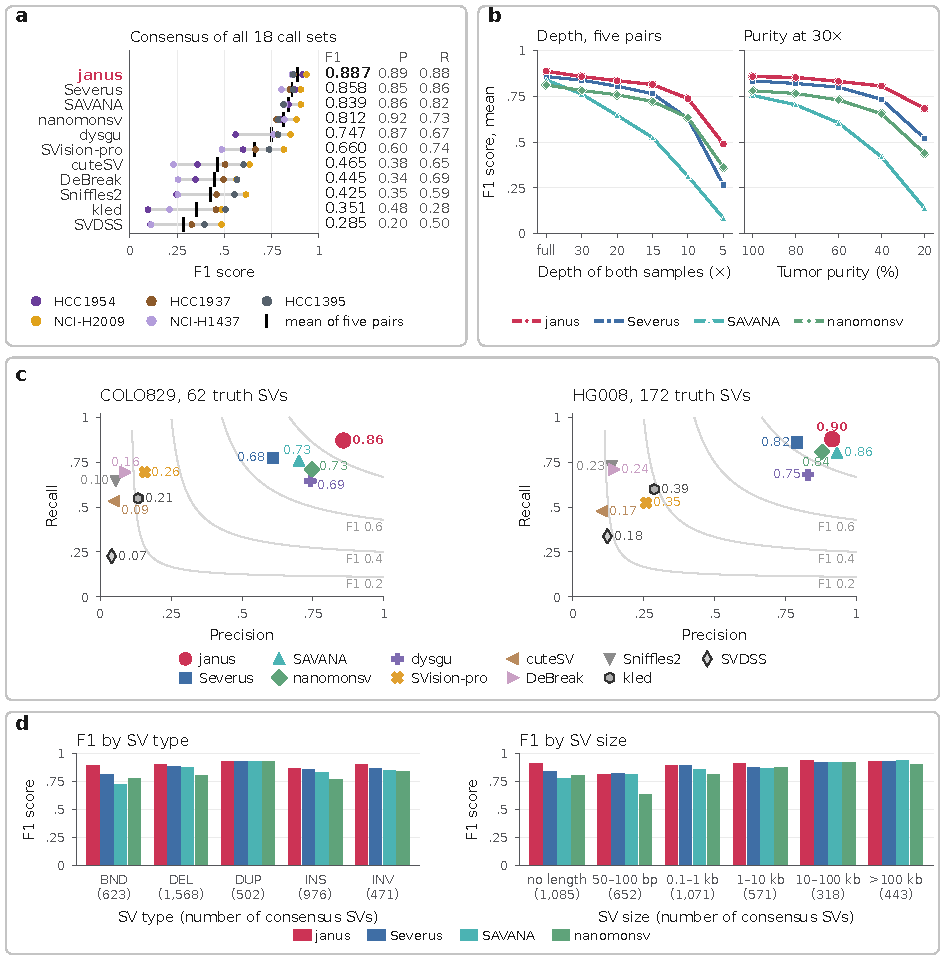
\includegraphics[width=157mm]{figures/fig_accuracy.pdf}
\caption{Accuracy of \tool and the other callers. (a) F1 score of the 11 PacBio HiFi call sets per CASTLE pair (dots) and the mean over pairs (bar), against the consensus of all 18 call sets and of the 17 other than \tool (P, precision; R, recall). (b, c) Precision and recall on COLO829 (b) and HG008 (c), with curves of equal F1 score. (d, e) F1 score by SV type (d) and size (e), five pairs pooled; inversions include inverted junctions; first size class: SVs without length; consensus SVs in parentheses. (f--i) F1 score (f, h) and precision and recall (g, i) at reduced depth (f, g) and purity (h, i).
Shading: bootstrap 95\% interval of \tool; above (f, h): bootstrap $p$-value against the best other caller, red if $p<0.05$.}
\label{fig:castle}
\end{figure}

Against the 18-caller consensus, \tool achieved the highest mean F1 score (0.881; Fig.~\ref{fig:castle}a, Fig.~\ref{supfig:allsets}), outperforming Severus (0.858 on HiFi, 0.843 on ONT), SAVANA (0.837), and nanomonsv (0.810). \tool ranked first in four pairs, trailing Severus only on HCC1395 (Fig.~\ref{fig:castle}a). ONT call sets for SAVANA and nanomonsv showed lower F1 scores and precision than their HiFi equivalents (Fig.~\ref{supfig:allsets}). Among Illumina tools, Manta (mean F1 0.600) and GRIPSS (0.565) surpassed ONT Sniffles2 (0.489) and five HiFi callers, whereas SvABA (0.403) exceeded only kled and SVDSS; all three performed best on HCC1954 and worst on NCI-H2009 (Table~\ref{suptab:allwith}). Finally, while nanomonsv attained the highest precision on HiFi data, \tool delivered the highest recall across all HiFi call sets (Fig.~\ref{supfig:allsets}).

Scoring all callers against the 17-caller consensus (excluding \tool from the truth set) placed Severus first on PacBio HiFi data (mean F1=0.859), narrowly ahead of \tool (0.857) and SAVANA (0.847; Fig.~\ref{fig:castle}a). Under a leave-one-caller-out benchmark, where no tool contributes to its own truth set, \tool led all five pairs with a mean F1 score of 0.857, surpassing Severus (0.832) and SAVANA (0.823; Section~\ref{supsec:loo}, Fig.~\ref{supfig:allsets}c).

To assess generalization, we evaluated two independent benchmarks outside the training set: COLO829 (melanoma, 62 validated SVs)~\cite{colo829} and HG008 (pancreatic tumor, GIAB draft benchmark v0.5 with 172 SVs)~\cite{hg008}. Trained on all five CASTLE pairs, \tool achieved the highest F1 score and recall among all PacBio HiFi callers on both datasets (Table~\ref{tab:external}, Fig.~\ref{fig:castle}b). On COLO829, \tool identified 54 SVs across 65 calls (F1 0.850), outperforming SAVANA (0.729), nanomonsv (0.727), dysgu (0.690), and Severus (0.681). On HG008, \tool attained an F1 score of 0.886, surpassing SAVANA (0.863), nanomonsv (0.842), and Severus (0.825).

Across pooled CASTLE pairs, \tool outperformed the four published HiFi callers for breakends, deletions, insertions, inversions, and SVs spanning 1--100\,kb. Conversely, SAVANA, Severus, and nanomonsv surpassed \tool on duplications; SAVANA and Severus led on SVs $>100$\,kb; Severus led on 0.1--1\,kb events; and both Severus and SAVANA outperformed \tool on 50--100\,bp variants (Fig.~\ref{fig:castle}c; Table~\ref{suptab:types}).



\begin{table}[tbp]
\centering
\caption{Experimental evaluation using PacBio HiFi datasets generated from COLO829 and HG008}
\label{tab:external}
\small
\resizebox{\ifdim\width>\textwidth\textwidth\else\width\fi}{!}{\begin{tabular}{lrrrrrrrr}
\toprule
 & \multicolumn{4}{c}{COLO829} & \multicolumn{4}{c}{HG008} \\
Caller & Calls & Precision & Recall & F1 & Calls & Precision & Recall & F1 \\
\midrule
\tool & 65 & \textbf{0.831} & \textbf{0.871} & \textbf{0.850} & 169 & 0.893 & \textbf{0.878} & \textbf{0.886} \\
SAVANA & 67 & 0.701 & 0.758 & 0.729 & 148 & \textbf{0.932} & 0.802 & 0.863 \\
nanomonsv & 59 & 0.746 & 0.710 & 0.727 & 158 & 0.880 & 0.808 & 0.842 \\
dysgu & 54 & 0.741 & 0.645 & 0.690 & 141 & 0.830 & 0.680 & 0.748 \\
Severus & 79 & 0.608 & 0.774 & 0.681 & 187 & 0.791 & 0.860 & 0.825 \\
SVision-pro & 275 & 0.156 & 0.694 & 0.255 & 348 & 0.259 & 0.523 & 0.346 \\
kled & 256 & 0.133 & 0.548 & 0.214 & 359 & 0.287 & 0.599 & 0.388 \\
DeBreak & 491 & 0.088 & 0.694 & 0.156 & 843 & 0.145 & 0.709 & 0.240 \\
Sniffles2 & 743 & 0.054 & 0.645 & 0.099 & 912 & 0.137 & 0.727 & 0.231 \\
cuteSV & 689 & 0.048 & 0.532 & 0.088 & 794 & 0.103 & 0.477 & 0.170 \\
SVDSS & 352 & 0.040 & 0.226 & 0.068 & 476 & 0.122 & 0.337 & 0.179 \\
\bottomrule
\end{tabular}}
\tabnotes{COLO829 (62 validated somatic SVs of at least 50\,bp) and HG008 (draft benchmark v0.5), scored with Minda; neither pair was part of the training data.
Rows ordered by F1 score on COLO829; bold: highest.}
\end{table}

We assessed caller robustness by downsampling both normal and tumor reads across all five CASTLE pairs to 30$\times$, 20$\times$, 15$\times$, 10$\times$, and 5$\times$, and by generating 30$\times$ mixtures spanning 100\% down to 20\% tumor purity. Scoring each run against its full-depth consensus, \tool substantially outperformed Severus, SAVANA, and nanomonsv under limited signal (Fig.~\ref{fig:castle}d; Section~\ref{supsec:depth}). Between 30$\times$ and 5$\times$ coverage, \tool's mean F1 score decreased from 0.856 to 0.476 (recall dropped from 0.863 to 0.387), whereas Severus declined more sharply from 0.838 to 0.264 as its recall fell to 0.164. At 20\% tumor purity, \tool maintained a mean precision of 0.870 and an F1 score of 0.679 across the five pairs, compared with 0.520 for Severus.

\begin{table}[tbp]
\centering
\caption{Call set accuracy comparison using PacBio HiFi datasets from the CASTLE panel}
\label{tab:callers}
\small
\setlength{\tabcolsep}{4pt}
\resizebox{\textwidth}{!}{%
\begin{tabular}{lrrrrrrrrrrrrr}
\toprule
 & \multicolumn{6}{c}{Consensus of 18 call sets} & \multicolumn{6}{c}{Consensus of 17 call sets, without \tool} & \\
\cmidrule(lr){2-7}\cmidrule(lr){8-13}
Caller & HCC1954 & NCI-H2009 & HCC1937 & NCI-H1437 & HCC1395 & Mean & HCC1954 & NCI-H2009 & HCC1937 & NCI-H1437 & HCC1395 & Mean & Time (h:mm) \\
\midrule
\tool     & \textbf{0.909} & \textbf{0.928} & \textbf{0.861} & \textbf{0.850} & 0.855 & \textbf{0.881} & 0.869 & \textbf{0.914} & 0.829 & \textbf{0.831} & 0.842 & 0.857 & \textbf{0:11} \\
Severus     & 0.873 & 0.905 & 0.846 & 0.799 & \textbf{0.866} & 0.858 & \textbf{0.886} & 0.904 & \textbf{0.848} & 0.798 & \textbf{0.861} & \textbf{0.859} & 6:24 \\
SAVANA      & 0.835 & 0.903 & 0.817 & 0.818 & 0.813 & 0.837 & 0.860 & 0.904 & 0.827 & 0.827 & 0.818 & 0.847 & 5:39 \\
nanomonsv   & 0.795 & 0.880 & 0.774 & 0.816 & 0.784 & 0.810 & 0.824 & 0.881 & 0.783 & 0.830 & 0.787 & 0.821 & 5:27 \\
dysgu       & 0.557 & 0.848 & 0.781 & 0.753 & 0.784 & 0.745 & 0.583 & 0.851 & 0.790 & 0.762 & 0.786 & 0.754 & 4:23 \\
SVision-pro & 0.597 & 0.815 & 0.664 & 0.486 & 0.739 & 0.660 & 0.608 & 0.817 & 0.664 & 0.485 & 0.738 & 0.662 & 4:44 \\
cuteSV      & 0.356 & 0.632 & 0.503 & 0.229 & 0.601 & 0.464 & 0.355 & 0.632 & 0.509 & 0.230 & 0.605 & 0.466 & 4:21 \\
DeBreak     & 0.346 & 0.563 & 0.495 & 0.253 & 0.566 & 0.445 & 0.355 & 0.564 & 0.497 & 0.254 & 0.569 & 0.448 & 4:25 \\
Sniffles2   & 0.245 & 0.613 & 0.459 & 0.251 & 0.553 & 0.424 & 0.254 & 0.615 & 0.463 & 0.253 & 0.555 & 0.428 & 4:22 \\
kled        & 0.095 & 0.485 & 0.455 & 0.210 & 0.504 & 0.350 & 0.099 & 0.489 & 0.464 & 0.213 & 0.510 & 0.355 & 4:21 \\
SVDSS       & 0.107 & 0.484 & 0.328 & 0.110 & 0.394 & 0.284 & 0.108 & 0.483 & 0.323 & 0.109 & 0.394 & 0.284 & 6:36 \\
\bottomrule
\end{tabular}}
\tabnotes{F1 score of \tool and of the callers we ran on the same PacBio HiFi reads, against the consensus of all 18 call sets and of the 17 call sets other than \tool (bold: best).
Time: wall clock on HCC1954 from the read sets to the calls on 16 threads (SAVANA on 8), including mapping (4:19) and, for Severus and SAVANA, phasing.}
\end{table}

%%%%%%%%%%%%%%%%%%%%%%%%%%%%
}

\subsection{Calling SVs in multiple tumors within one personal pangenome}\label{sec:multiple}
\begin{figure}[!htb]
\centering
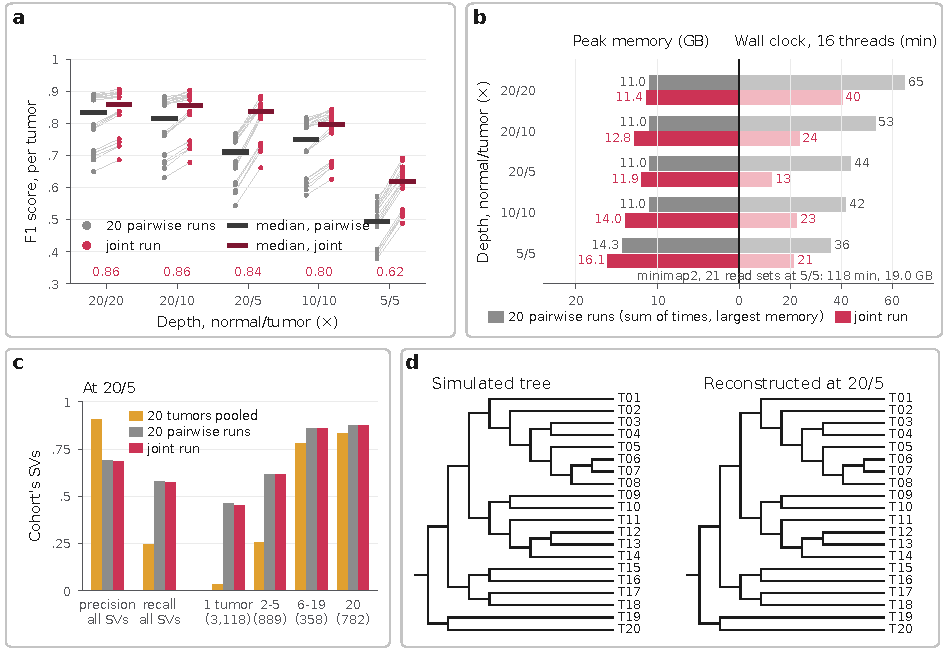
\includegraphics[width=0.9\textwidth]{figures/fig_sim.pdf}
\caption{A simulated case with one normal and 20 tumors at five normal/tumor depths. (a) F1 score per tumor for the pairwise runs and the joint run with the clade pass; bars: medians over the 20 tumors; numbers: median of the joint run. (b) Wall-clock time from the packed reads on 16 threads and peak memory of the pairwise runs (sum of the times, largest memory) and of the joint run, labeled by depth. (c) Precision and recall over the cohort's 5,147 distinct SVs at 20/5, and recall by the number of tumors carrying the SV: the 20 tumors pooled into one sample, the pairwise runs together, and the joint run. (d) The simulated tree and the tree reconstructed from the first-pass joint calls at 20/5.}
\label{fig:sim}
\end{figure}


Due to the lack of multi-sample long-read tumor--normal cohorts with established ground truth, we evaluated joint calling on simulated data~\cite{Battistella_2025,msprime,badread}: one normal genome with real germline variants~\cite{hgsvc3} and 20 lineage-related tumor clones that inherit ancestral somatic SVs (Section~\ref{supsec:simgen}). Across the 5,147 total simulated SVs, individual tumors harbor 1,016--1,353 variants (Fig.~\ref{supfig:simgen}). We simulated 20$\times$ PacBio HiFi reads per genome and downsampled to 10$\times$ and 5$\times$ across five normal/tumor depth configurations (Table~\ref{suptab:sim}): uniform moderate depth (20/20$\times$), uniform low depth (10/10$\times$, 5/5$\times$), and asymmetric designs (20/10$\times$, 20/5$\times$). We evaluated call sets against simulated junction coordinates using a 500\,bp tolerance and 50\,bp minimum size (Section~\ref{supsec:simeval}).

We evaluated joint calling across the 20 simulated tumors in two modes: 20 separate pairwise runs against the normal sample and a single joint run spanning all 21 read sets. At 20/5$\times$ coverage, joint calling increased the median F1 score across all clones from 0.712 to 0.839 (Tables~\ref{suptab:sim} and~\ref{suptab:simtumor}, Fig.~\ref{fig:sim}a), driven primarily by recall (0.584 to 0.767) alongside modest precision gains (0.910 to 0.918). Joint calling maintained superior median F1 scores across all depths, though the advantage narrowed at 20/20$\times$ (0.860 versus 0.835). The gain comes largely from cross-sample classification, which rescues candidates confirmed with high confidence in another tumor (Methods): the first pass alone reached 0.796 at 20/5$\times$, and the clade pass added the rest, reporting 7,078 carriers of which 96\% were true (Table~\ref{suptab:clade}). The joint run at 20/5$\times$ thus reached the median F1 score of separate runs at 20/20$\times$ (0.839 versus 0.835) with a quarter of the tumor reads. Pooling the 20 tumors into one 100$\times$ sample instead, the bulk alternative to a joint run, found 1,272 of the cohort's 5,147 distinct SVs at 20/5$\times$, against 2,951 for the joint run (Fig.~\ref{fig:sim}c, Table~\ref{suptab:pooled}): the pool recovered the SVs shared by six or more tumors nearly as well (0.78 versus 0.86) but only 4\% of the 3,118 private SVs, against 45\% for the joint run. Its higher precision (0.905 versus 0.685) follows from the same selectivity: a private SV has a 5\% share of the pooled reads, which the classifier scores as an artifact, so the pool calls only the shared SVs, whereas the false calls of the joint run are mostly records of a single tumor at 5$\times$ (Table~\ref{suptab:pooled}). Starting from packed reads, the joint run processed all 20 tumors in 12.8\,min, 3.4$\times$ faster than the aggregated pairwise runs (43.7\,min; Fig.~\ref{fig:sim}b), with only a minor memory increase over the largest pairwise run (11.9 versus 11.0\,GB at 20/5$\times$; Fig.~\ref{fig:sim}b). In contrast, reference alignment and sorting via minimap2 required 1\,h 58\,min at 5/5$\times$ and an extrapolated 7.7\,h at 20/20$\times$ prior to variant calling.

The first-pass calls at 20/5$\times$ yielded 5,873 unique SVs (1,846 false positives, with 1,730 restricted to single tumors), and a neighbor-joining tree~\cite{nj,ape} built on their pairwise SV differences recovered all 17 simulated splits (Robinson--Foulds distance 0~\cite{rf}; Fig.~\ref{fig:sim}d), as did the trees reconstructed at the other four depth settings (Table~\ref{suptab:sim}).

\begin{figure}[!htb]
\centering
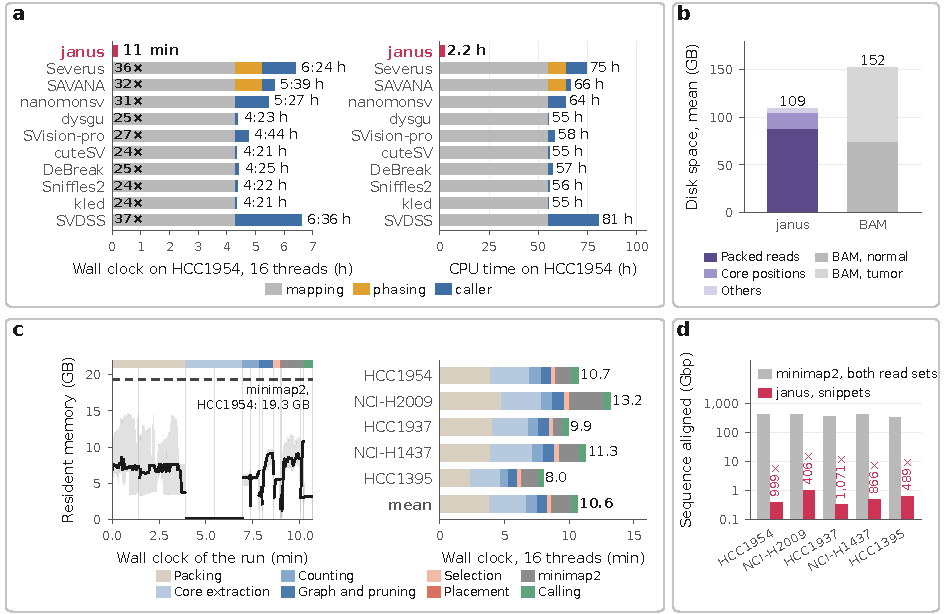
\includegraphics[width=\textwidth]{figures/fig_runtime.pdf}
\caption{Computational cost of \tool and of the alignment-based pipelines on 16 threads (SAVANA on 8 threads). (a) Wall-clock time (left) and CPU time (right) from the read sets to the calls on HCC1954, with the factor relative to \tool. (b) Disk use, mean of the five pairs. (c) Resident memory over a run of \tool: median (line) and range (band) of the five pairs; strip: stages, each step as wide as its median duration; dashed: minimap2 peak on HCC1954; right: wall-clock time of \tool by stage, per pair and as the mean of the five pairs. (d) Sequence aligned per pair: both read sets for minimap2, snippets for \tool.}
\label{fig:runtime}
\end{figure}

\subsection{Runtime and memory per pair}\label{sec:runtime}

Mapping both read sets of HCC1954 with minimap2 and sorting the alignments took 4 h 19 min with a peak memory of 19.3\,GB, and the complete \tool run on this pair needed about 4\% of this time (Table~\ref{suptab:mapping}, Section~\ref{supsec:compute}) and 56\% of this memory (10.9\,GB). With variant calling included, the alignment-based pipelines took at least 4 h 21 min (cuteSV and kled). Severus and SAVANA each spent 56 min of their run time on phasing using Clair3~\cite{clair3} and LongPhase~\cite{longphase} (Table~\ref{suptab:pipelines}, Fig.~\ref{fig:runtime}a). The minimap2 alignment required a peak memory of 10.8--12.1\,GB when aligning the snippets or their unaligned parts, whereas the other steps of \tool used up to 9.7\,GB (Fig.~\ref{fig:runtime}c, Table~\ref{suptab:time}). On disk, the intermediate files of \tool require 90--121\,GB per pair, most of this space for the packed reads, whereas the two sorted BAM files needed by the alignment-based callers require 117--167\,GB, which is on average 39\% more (Fig.~\ref{fig:runtime}b; Section~\ref{supsec:files}, Table~\ref{suptab:files}). 
Starting from the FASTQ files, \tool took 8 to 13 minutes per pair (Table~\ref{suptab:time}, Fig.~\ref{fig:runtime}c). The snippets that \tool aligned amounted to 0.34--1.02\,Gbp per pair, which is 0.09--0.25\% of the 309--420\,Gbp of the two read sets of the same pair (Fig.~\ref{fig:runtime}d); \tool did not align any read of the normal sample. 

% this is confusing, is this a single-cpu time? we probably dont need this here
%End-to-end, \tool used 2.2 h on HCC1954, whereas mapping alone used 55 h and the complete pipelines of the other callers used 55--81 h (Fig.~\ref{fig:runtime}a).

